\documentclass[tikz,border=4pt]{standalone}

\usepackage{amsmath}
\usepackage{amssymb}
\usepackage{xcolor}
\usepackage{tikz}


\usetikzlibrary{
    arrows,
    arrows.meta,
    automata,
    backgrounds,
    calc,
    decorations.pathreplacing,
    fit,
    matrix,
    positioning,
    shapes,
    shapes.arrows,
    shapes.geometric,
    shapes.multipart
}



\tikzset{
  start/.style={
    rectangle,
    rounded corners,
    minimum width=3.5cm,
    minimum height=1cm,
    text centered,
    text width=3cm,
    draw=black,
    fill=green!20
  },
  stop/.style={
    rectangle,
    rounded corners,
    minimum width=3cm,
    minimum height=1cm,
    text centered,
    text width=2.5cm,
    draw=black,
    fill=red!20
  },
  decision/.style={
    diamond,
    aspect=2,
    minimum width=3cm,
    minimum height=1.2cm,
    text centered,
    text width=2.5cm,
    inner sep=1pt,
    draw=black,
    fill=yellow!20
  },
  process/.style={
    rectangle,
    minimum width=3cm,
    minimum height=1cm,
    text centered,
    text width=2.7cm,
    draw=black,
    fill=blue!10
  },
  arrow/.style={
    thick,
    -{Stealth}
  }
}


\usetikzlibrary{
  arrows.meta,
  positioning,
  shapes.geometric
}

\tikzset{
  start/.style={
    rectangle,
    rounded corners,
    minimum width=3.5cm,
    minimum height=1cm,
    text centered,
    text width=3cm,
    draw=black,
    fill=green!20
  },
  stop/.style={
    rectangle,
    rounded corners,
    minimum width=3cm,
    minimum height=1cm,
    text centered,
    text width=2.5cm,
    draw=black,
    fill=red!20
  },
  decision/.style={
    diamond,
    aspect=2,
    minimum width=3cm,
    minimum height=1.2cm,
    text centered,
    text width=2.5cm,
    inner sep=1pt,
    draw=black,
    fill=yellow!20
  },
  io/.style={
    trapezium,
    trapezium left angle=70,
    trapezium right angle=110,
    minimum width=3.5cm,
    minimum height=1cm,
    text centered,
    text width=3cm,
    draw=black,
    fill=blue!20
  },
  arrow/.style={
    thick,
    -{Stealth}
  }
}


\begin{document}

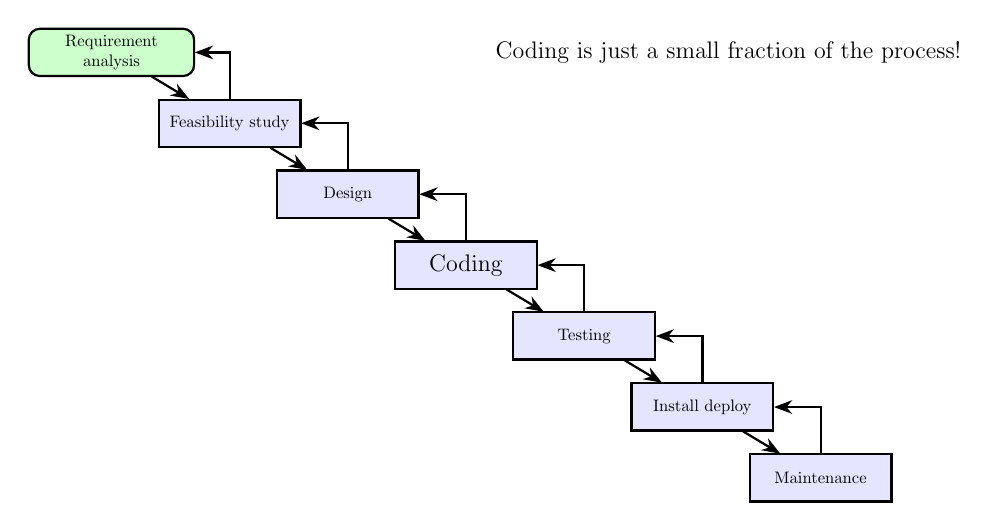
\begin{tikzpicture}[node distance=1.5cm, thick,scale=1.6, every node/.style={scale=0.6}]
    \node (ra) [start] {Requirement analysis};
    \node (fs) [process, below of=ra, xshift=2.5cm] {Feasibility study};
    \node (de) [process, below of=fs, xshift=2.5cm] {Design};
    \node (co) [process, below of=de, xshift=2.5cm] {\Large Coding};
\node (ts) [process, below of=co, xshift=2.5cm] {Testing};
    \node (id) [process, below of=ts, xshift=2.5cm] {Install deploy};
    \node (mn) [process, below of=id, xshift=2.5cm] {Maintenance};
    
    \draw [arrow] (ra) -- (fs);
    \draw [arrow] (fs) -- (de);
    \draw [arrow] (de) -- (co);
    \draw [arrow] (co) -- (ts);
    \draw [arrow] (ts) -- (id);
    \draw [arrow] (id) -- (mn);
    
    \draw[arrow] (mn) |- (id);
    \draw[arrow] (id) |- (ts);
    \draw[arrow] (ts) |- (co);
    \draw[arrow] (co) |- (de);
    \draw[arrow] (de) |- (fs);
    \draw[arrow] (fs) |- (ra);

\draw (3, 0) node[anchor=west] {\Large Coding is just a small fraction of the process!};
  \end{tikzpicture}

\end{document}
